\documentclass[11pt, letterpaper]{article}
\setlength{\parindent}{0in}
\setlength{\textheight}{8.7in}
\setlength{\textwidth}{6.8in}
\setlength{\oddsidemargin}{-0.3in}
\setlength{\evensidemargin}{0.0in}
\addtolength{\topmargin}{-1in}
\setlength{\parskip}{0.1in}

\usepackage{amsmath, amsfonts, amssymb, color}
\usepackage{bm}
\usepackage{booktabs}
\usepackage{enumerate}
\usepackage{graphicx}
\usepackage{pdfpages}
\newcommand*{\justifyheading}{\raggedleft}


\renewcommand{\baselinestretch}{1.0}

\newcommand{\bx}{{\bm x}}
\newcommand{\bX}{{\bm X}}
\newcommand{\by}{{\bm y}}
\newcommand{\bY}{{\bm Y}}
\newcommand{\bW}{{\bm W}}
\newcommand{\bG}{{\bm G}}
\newcommand{\bR}{{\bm R}}
\newcommand{\bZ}{{\bm Z}}
\newcommand{\bV}{{\bm V}}
\newcommand{\bL}{{\bm L}}
\newcommand{\bz}{{\bm z}}
\newcommand{\be}{{\bm e}}
\newcommand{\bgamma}{{\bm \gamma}}
\newcommand{\bbeta}{{\bm \beta}}
\newcommand{\balpha}{{\bm \alpha}}
\newcommand{\bSigma}{{\bm \Sigma}}
\newcommand{\bmu}{{\bm \mu}}
\newcommand{\btheta}{{\bm \theta}}
\newcommand{\bepsilon}{{\bm \epsilon}}
\newcommand{\bone}{{\bm 1}}
\newcommand{\bzero}{{\bm 0}}
\newcommand{\bC}{{\bm C}}
\newcommand{\bI}{{\bm I}}
\newcommand{\bA}{{\bm A}}
\newcommand{\bB}{{\bm B}}
\newcommand{\bQ}{{\bm Q}}
\newcommand{\bS}{{\bm S}}
\newcommand{\bD}{{\bm D}}
\newcommand{\cQ}{\mathcal{Q}}
\newcommand{\cU}{\mathcal{U}}
\newcommand{\cI}{\mathcal{I}}
\newcommand{\cL}{\mathcal{L}}

\newcommand{\beas}{\begin{eqnarray*}}
\newcommand{\eeas}{\end{eqnarray*}}

\newenvironment{equationarrayright}{
                          \begin{eqnarray*}
                          \begin{array}{rcll}
                         }{
                          \end{array}
                          \end{eqnarray*}
                         }
\newcommand{\bear}{\begin{equationarrayright}}
\newcommand{\eear}{\end{equationarrayright}}

\renewcommand\arraystretch{1.3}

\DeclareMathOperator*{\argmin}{arg\,min}

\title{STAT/BIOST 571: Homework 6}
\author{Philip Pham}
\date{\today}

\begin{document}

\maketitle

\section*{Problem 1: Fitting and interpreting the results of a linear mixed effects model; robust standard error estimation (20 points)}
 
{\em Download the $\texttt{creatinine.csv}$ dataset from the course website.  This file
contains repeated observational data for 619 subjects, some of whom have hypertension and some
of whom have a hereditary kidney disease, as indicated by the \texttt{group} variable, according to the coding in the Table~\ref{ta:orig.hw1}.
\begin{table}[ht]
\centering
\begin{tabular}{cccc}
\toprule
Group&Kidney disease&Hypertension&Sample size\\
\midrule
1&Yes&Yes&294\\
2&Yes&No&103\\
3&No&Yes&73\\
4&No&No&149\\
\bottomrule
\end{tabular}
\caption{Measurements of serum creatinne reciprocals from 619 subjects in four groups}
\label{ta:orig.hw1}
\end{table}
The outcome variable is \texttt{scr}, the reciprocal of
serum creatinine.  Serum creatinine is a measure of kidney function, with lower values
indicating better kidney function.  Higher values of the reciprocal reported in \texttt{scr} indicate better kidney function.  The observations were taken at arbitrary times from each subject, with the number
of observations ranging from 1 to 22.  Ignoring hypertension status, we are interested in estimating
the rate of change of \texttt{scr} for subjects with and without hereditary kidney disease.
Thus, the only fixed effect covariates in your model should be age, kidney disease status, and possibly an
interaction between these. 
In order to account for correlation within subjects, you will be fitting a linear mixed effects model with
uncorrelated random slopes and intercepts and serial correlation of residuals that follows a spherical
correlation model, including a nugget (correlation should be based on the timing of observations).  Please use the \texttt{lme()} function in the \texttt{nlme} package in R to fit your models (i.e., do not code your own nonlinear optimization).}
\begin{enumerate}[(a)]
\item {\em Fit the model by ML and
report the
estimated values of all variance parameters. }

\begin{table}
  \centering
  \begin{tabular}{lrr}
    \toprule
    & \multicolumn{2}{c}{Model} \\
    Parameter & Without interaction (Equation \ref{eqn:mean_model_no_interaction}) & With interaction (Equation \ref{eqn:mean_model_interaction}) \\
    \midrule
    $\hat{\sigma}$ & 0.2633414 & 0.225834 \\
    $\hat{\sigma}_{\gamma_0}$ & 0.04643211 & 0.1317468 \\
    $\hat{\sigma}_{\gamma_1}$ & 0.00522239 & 0.004823202 \\
    $\hat{\alpha}_r$ & 7.8894707 & 4.6700641 \\
    $\hat{\alpha}_n$ & 0.1759323  & 0.2299764 \\
    \bottomrule
  \end{tabular}
  \caption{Variance parameters for ML-fitted models.}
  \label{tab:variance_parameters}
\end{table}

\begin{description}
  The parameter estimates of fitting the model without and with an interaction
  term can be seen in Tables \ref{tab:standard_errors_no_interaction} and
  \ref{tab:standard_errors_interaction}. The variance parameters can be found in
  Table \ref{tab:variance_parameters}. Their meaning is detailed in the
  subsequent paragraphs. The \textsf{R} model summaries can be found in the
  Appendix.

  Let $t_{ij}$ be the age of the subject $i$ at observation $j$. Let $x_i$
  indicate whether the subject has has kidney disease. Without an interaction
  term, the mean model is
  \begin{equation}
    Y_{ij} = \left(\beta_0 + \gamma_0\right) +
    \beta_2x_i +
    \left(\beta_1 + \gamma_1\right)t_{ij} + \epsilon_{ij}.
    \label{eqn:mean_model_no_interaction}
  \end{equation}
  With the interaction term, the mean model is
  \begin{equation}
    Y_{ij} = \left(\beta_0 + \gamma_0\right) +
    \beta_2x_i +
    \left(\beta_1 + \beta_3x_i +\gamma_1\right)t_{ij} + \epsilon_{ij}.
    \label{eqn:mean_model_interaction}
  \end{equation}
  $\gamma_j$ are the random effects, where $\gamma_0$ is subject-specific
  adjustment to the intercept, and $\gamma_1$ is the subject-specific adjustment
  to the slope.
  
  The covariance structure of a cluster $i$ can be described by the matrix
  \begin{equation}
    \Sigma_i = \sigma^2\left(Z_iGZ_i^\intercal + R_i\right)
    \label{eqn:cluster_covariance}
  \end{equation}
  $Z_i$ is a $m_i \times 2$ matrix, where the first column entries are all $1$s,
  and the second column entries are ages for each subject $t_{ij}$.

  $G$ is a $2 \times 2$ diagonal matrix that describes the variance of the
  random effects $\gamma_0$ and $\gamma_1$:
  \begin{equation}
    G = \frac{1}{\sigma^2}\begin{pmatrix}
      \sigma^2_{\gamma_0} & 0 \\
      0 & \sigma^2_{\gamma_1}
    \end{pmatrix}
    \label{eqn:random_effects_covariance}
  \end{equation}

  $R_i$ is an $m_i \times m_i$ matrix that describes the correlations between
  the $\epsilon_{ij}$s for different $j$s with a nugget parameter
  $0 \leq \alpha_n < 1$ and range parameter $\alpha_r > 0$. $R_{ijj} = 1$ and
  $R_{ijj^\prime} = \left(1 - \alpha_n\right) \exp\left(-\frac{\left\lvert
        t_{ij} - t_{ij^\prime}\right\rvert}{\alpha_r}\right)$. Estimates for
  these parameters can be found in Table \ref{tab:variance_parameters}.
\end{description}

\item {\em  Report point estimates and standard errors for all fixed effect
coefficients in your model.  Include three versions of standard error estimates: (i) robust/empirical sandwich SEs that correctly
account for clustering of the data, (ii) bootstrap SEs that correctly account for clustering of the data, and (iii) model based SE estimates based on the assumed random effect model being correct.}

% latex table generated in R 3.5.2 by xtable 1.8-3 package
% Sun Feb 24 15:29:24 2019
\begin{table}[ht]
\centering
\begin{tabular}{rrrr}
  \toprule
 & ML Standard Error & Sandwich Standard Error & Bootstrap Standard Error \\ 
  \midrule
(Intercept) & 0.039557 & 0.039348 & 0.039110 \\ 
  age & 0.000964 & 0.000941 & 0.000946 \\ 
  kidney.disease & 0.026260 & 0.025027 & 0.035603 \\ 
   \bottomrule
\end{tabular}
\caption{Standard error estimates for fixed effect parameters.} 
\label{tab:standard_errors_no_interaction}
\end{table}


\begin{description}
\item[Solution:] See Table \ref{tab:standard_errors_no_interaction} for the
  standard errors.

  Let $\hat{V}_i$ be the result of substituting the variance parameter estimates
  in Table \ref{tab:variance_parameters} into Equation
  \ref{eqn:cluster_covariance}. Let $W_i = \hat{V}_i^{-1}$ be the weight matrix
  for each cluster. Let $X_i$ be the matrix of cluster covariates, $1$s in the
  first column, age in the second column, and an indicator for kidney disease in
  the third column. Let $Y_i$ be the cluster response.

  If we assume the random effect model is correct, then the covariance matrix
  for the paramter estimates $\hat{\beta}$ is
  \begin{equation}
    \hat{\operatorname{var}}\left(\hat{\beta}\right)
    = \left(\sum_{i=1}^n X_i^\intercal W_iX_i\right)^{-1},
    \label{eqn:ml_variance}
  \end{equation}
  and we take the square root of the diagonals to obtain the standard errors for
  the ML Standard Error column.

  For the sandwich standard errors, we use the covariance matrix
  \begin{equation}
    \small
    \hat{\operatorname{var}}\left(\hat{\beta}\right)
    = \left(\sum_{i=1}^n X_i^\intercal W_iX_i\right)^{-1}
    \left(\sum_{i=1}^n X_i^\intercal W_i
      \left(Y_i - X_i\hat{\beta}\right)
      \left(Y_i - X_i\hat{\beta}\right)^\intercal
      W_iX_i\right)
    \left(\sum_{i=1}^n X_i^\intercal W_iX_i\right)^{-1},
    \label{eqn:sandwich_variance}
  \end{equation}
  which we use to get the Sandwich Standard Error column.

  For the bootstrap standard errors, we resample clusters, and then fit a model
  to the resampled clusters to get samples
  $\hat{\beta}^{(1)}, \hat{\beta}^{(2)},\ldots,\hat{\beta}^{(L)}$. In this case,
  $L = 2^{10}$. Then, $\hat{\operatorname{var}}\left(\hat{\beta}\right)$ is
  estimated by taking the unbiased covariance estimate of the samples. Taking
  the square root of the diagonals gives us the Bootstrap Standard Error column.

  In this case, the standard errors assuming the model is correct and the
  sandwich standard errors are very similar with the sandwich standard errors
  being slightly smaller. The bootstrap standard errors are largest. The
  difference is more than just Monte Carlo error, particularly for $\beta_2$ the
  coefficient for kidney disease, which hints at its interaction with other
  covariates.
\end{description}

\item {\em  Now, give point estimates and three versions of standard error estimates for the marginal rates of change in \texttt{scr} in subjects with and without 
kidney disease.  As in part (b), your three versions of SE estimates should be:  (i) robust/empirical sandwich SEs that correctly
account for clustering of the data, (ii) bootstrap SEs that correctly account for clustering of the data, and (iii) model based SE estimates based on the assumed random effect model being correct.  Depending on how you parameterized your model, these answers may or may not 
coincide with estimates you reported in part (b).  You may parameterize the model any way you wish,
but you must answer this question based on the output of a single call to \texttt{lme()}.}

% latex table generated in R 3.5.2 by xtable 1.8-3 package
% Tue Feb 26 08:35:18 2019
\begin{table}[ht]
\centering
\begingroup\small
\begin{tabular}{rrrrr}
  \toprule
 & Estimate & ML Standard Error & Sandwich Standard Error & Bootstrap Standard Error \\ 
  \midrule
(Intercept) & 1.190676 & 0.054232 & 0.050269 & 0.050770 \\ 
  age & -0.003108 & 0.001436 & 0.001194 & 0.001217 \\ 
  kidney.disease & 0.313575 & 0.071373 & 0.068325 & 0.070047 \\ 
  age:kidney.disease & -0.016649 & 0.001857 & 0.001705 & 0.001706 \\ 
   \bottomrule
\end{tabular}
\endgroup
\caption{Standard error estimates for fixed effect parameters with interaction term.} 
\label{tab:standard_errors_interaction}
\end{table}


\begin{description}
\item[Solution:] Table \ref{tab:standard_errors_interaction}
\end{description}

\end{enumerate}

\section*{Appendix}

Code for fitting models and generating tables is attached on the subsequent
pages.

\clearpage
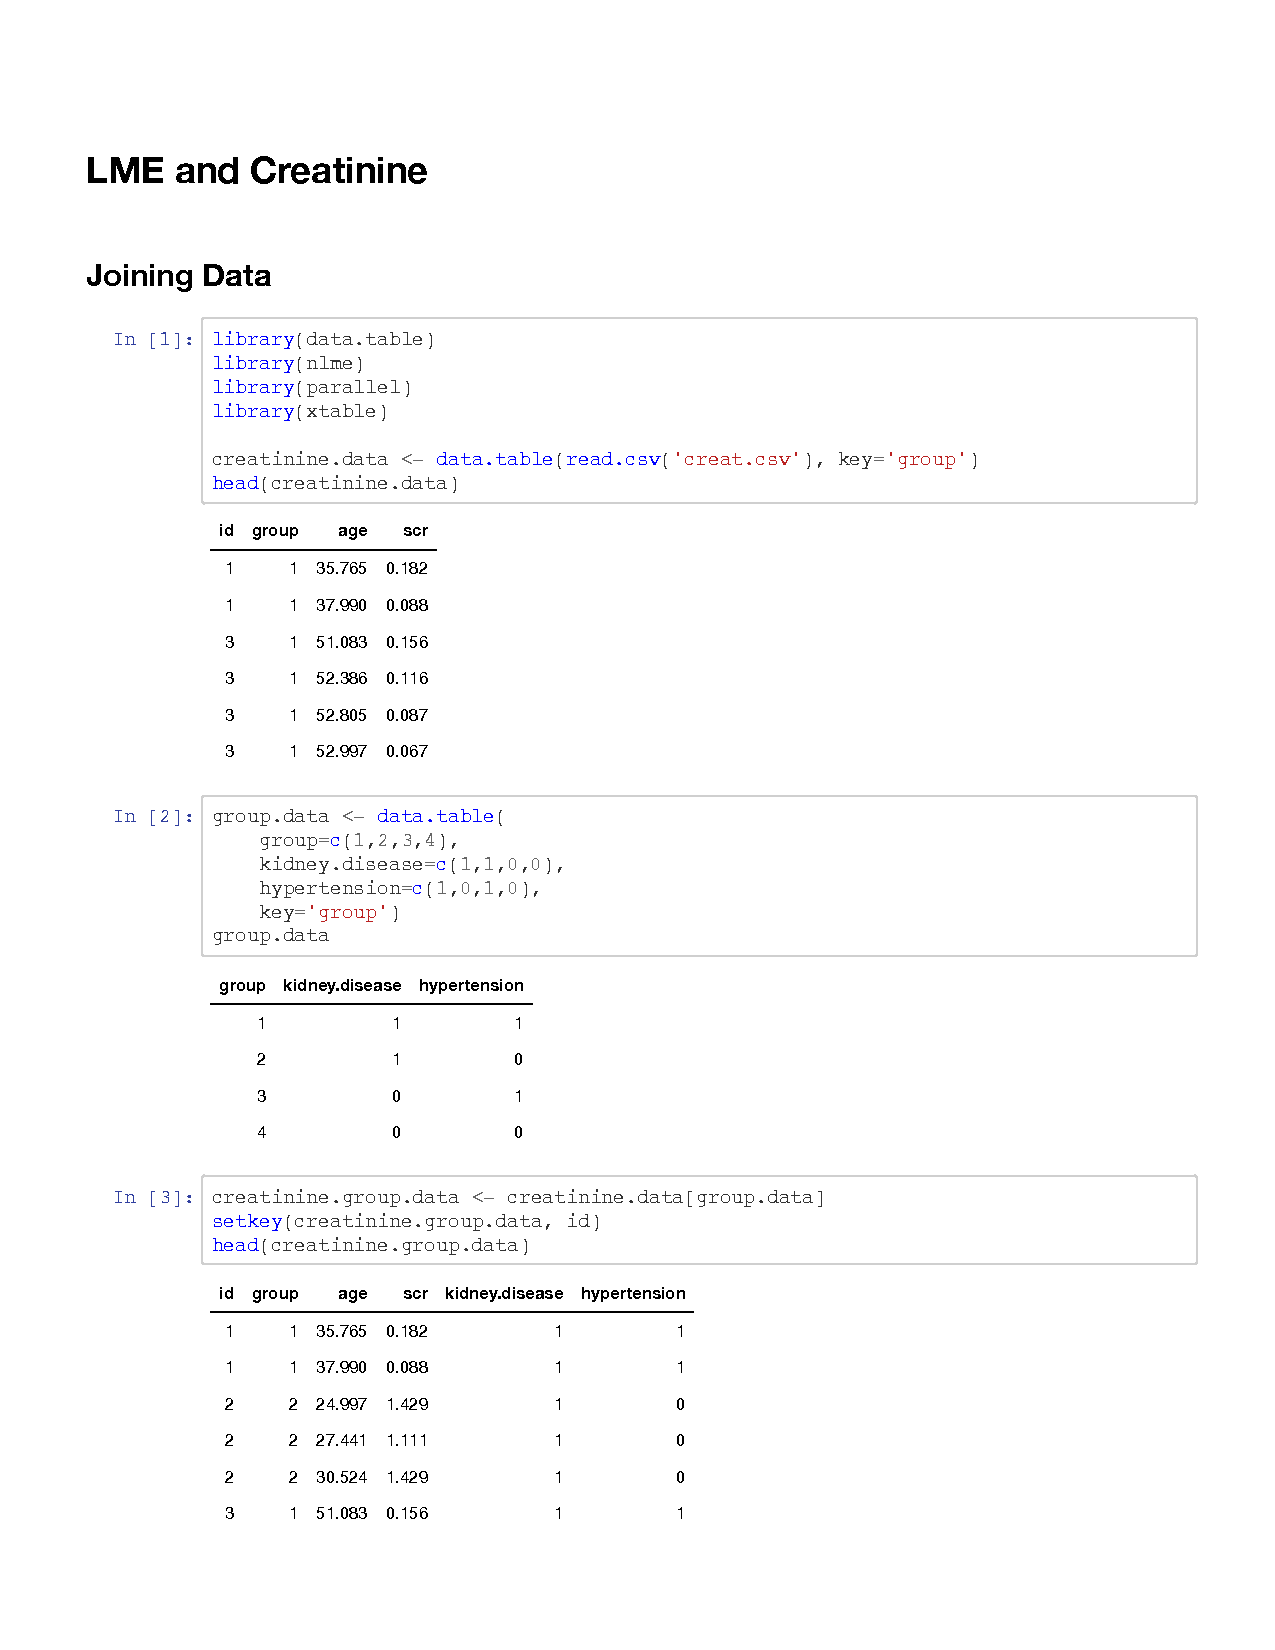
\includepdf[pages=-]{creatinine.pdf}

\end{document}